\section{MRG方法实现}

\begin{frame}{MSG与MRG}
    \begin{columns}
        \begin{column}{0.50\textwidth}
            \begin{block}{MSG}
                \begin{itemize}
                    \item 为了提取多尺度的模式,一种简单有效的方法是对于每层的点云都采用多个尺寸的局部区域进行特征聚合
                \end{itemize}
            \end{block}
            \begin{block}{MRG}
                \begin{itemize}
                    \item MSG方法计算成本较高,替代方法MRG通过连接不同层特征,在减少计算成本的同时仍保留多尺度模式提取能力
                \end{itemize}
            \end{block}
        \end{column}
        \begin{column}{0.50\textwidth}
            \begin{figure}
                \centering
                \includegraphics[width=0.6\textwidth]{doc/img/MRG与MSG.png}
                \caption{MSG与MRG}
                \label{fig:MSG-MRG}
            \end{figure}
        \end{column}
    \end{columns}
\end{frame}

\begin{frame}{使用MRG的分类网络结构}
    \begin{columns}
        \begin{column}{0.50\textwidth}
            \begin{block}{}
                \begin{itemize}
                    \item 论文并没有给出MRG方法的源码,我们根据论文中给出的网络结构实现了使用MRG的分类pointnet++
                    \item 右图是论文中的pointnet++的网络结构
                \end{itemize}
            \end{block}
        \end{column}
        \begin{column}{0.50\textwidth}
            \begin{figure}
                \centering
                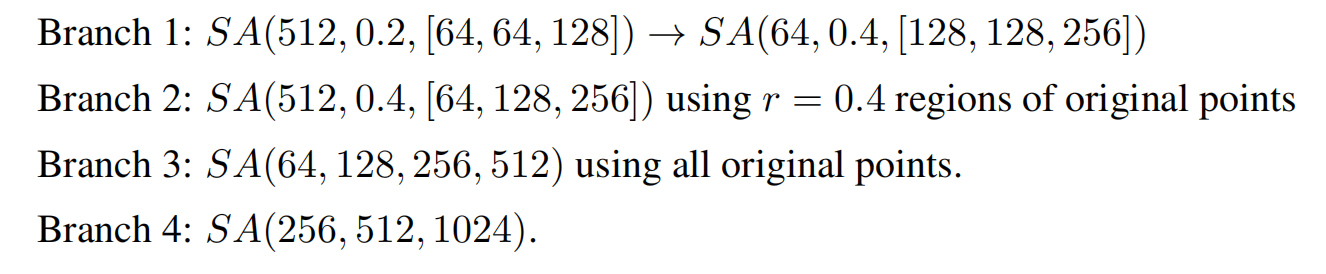
\includegraphics[width=0.9\textwidth]{doc/img/论文网络结构.png}
                \caption{MRG分类网络结构}
                \label{fig:structure}
            \end{figure}
        \end{column}
    \end{columns}
\end{frame}
\begin{frame}{使用MRG的分类网络结构}
    \begin{columns}
        \begin{column}{1\textwidth}
            \begin{block}{}
                \begin{itemize}
                    \item SA为Set Abstraction;(N,D)表示输入点数为N,特征维度为D;C表示连接操作
                \end{itemize}
            \end{block}
            \begin{figure}
                \centering
                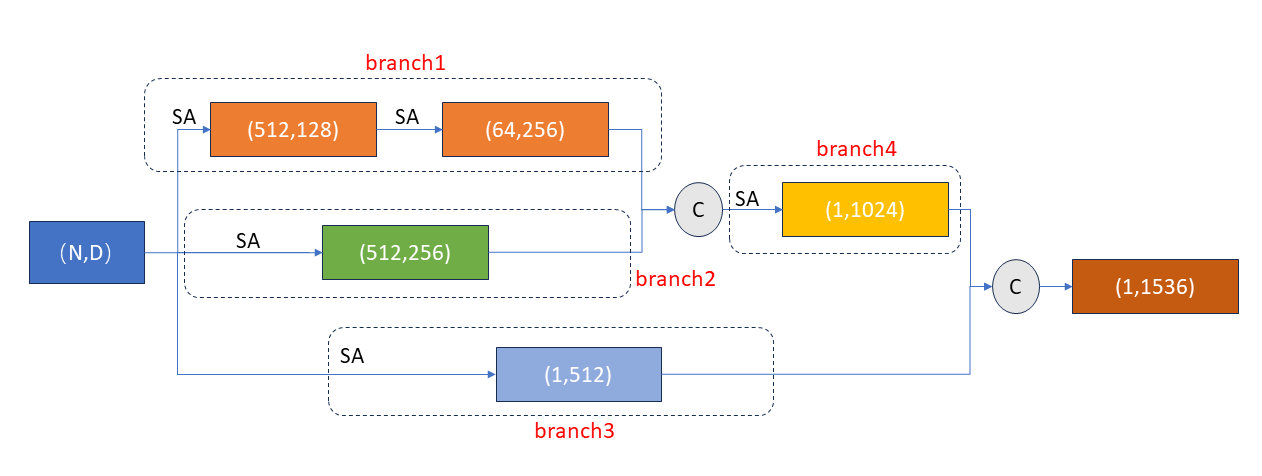
\includegraphics[width=0.8\textwidth]{doc/img/网络示意图.png}
                \caption{特征提取过程示意图}
                \label{fig:network}
            \end{figure}
        \end{column}
    \end{columns}
\end{frame}